\documentclass[sigconf]{acmart}

\usepackage{amsmath}
\usepackage{tikz}
\usetikzlibrary{arrows.meta,positioning,fit,calc}

\setcopyright{none}
\settopmatter{printacmref=false}
\renewcommand\shortauthors{Skaperdas et al.}

\title{OG-NSD: Neuro-Symbolic Ontology Drafting from Natural-Language Requirements}

\author{Efstratios Skaperdas}
\author{Kristi Cami}
\author{Nick Bassiliades}
\affiliation{%
  \institution{Department of Informatics, Aristotle University of Thessaloniki, Greece}%
  \country{Greece}}

\begin{document}

\begin{abstract}
Natural-language requirements are easy for analysts and domain stakeholders to write, but difficult to validate systematically and to transform into machine-interpretable semantic artifacts. We present \emph{OG-NSD}, a neuro-symbolic pipeline for ontology drafting from natural-language requirements. The pipeline combines LLM-based drafting with ontology-aware prompting, SHACL validation, OWL/DL reasoning, competency-question evaluation, and an iterative repair loop that converts symbolic violations into corrective prompts. We evaluate the approach through a controlled pilot study spanning neural baselines, a validation-oriented baseline, ontology-aware drafting, iterative repair policies, cross-domain transfer, and CQ-oriented iterative analysis. The results show a deliberately mixed but informative picture. Low-temperature drafting provides a strong raw baseline ($F1 = 0.4769$, 11/21 competency questions), ontology-aware prompting improves vocabulary alignment but not necessarily precision, and iterative repair helps only when conservative stopping policies are used. Among the tested repair strategies, the \texttt{max\_only} configuration yields the best balance within the iterative family ($F1 = 0.3427$, 11/21 competency questions), whereas aggressive CQ-driven repair leads to graph explosion and unstable reasoning. These findings support the main claim of the paper: symbolic feedback is most useful when treated as an active control mechanism for ontology drafting rather than as a purely post-hoc diagnostic layer.
\end{abstract}

\keywords{LLMs, ontology engineering, requirements formalization, neuro-symbolic AI, SHACL, OWL}

\maketitle

\section{Introduction}

Requirements are commonly expressed in natural language because this format is accessible to analysts, developers, and domain stakeholders. However, natural-language requirements are often ambiguous, underspecified, and difficult to validate systematically. This limits downstream automation, including traceability, consistency checking, reuse, and formal analysis. In ontology engineering, the problem is particularly significant: requirement documents may implicitly define classes, relations, hierarchies, and domain constraints, yet converting them into formal semantic artifacts remains a labor-intensive and expert-driven task \cite{gruber1993,uschold1996}.

Large language models (LLMs) have recently shown strong capabilities for extracting structured information from free text and producing draft knowledge representations. This raises a natural question: can LLMs accelerate ontology drafting directly from requirement descriptions? The answer is promising, but not straightforward. In practice, LLM outputs may omit constraints, invent classes or properties, drift away from domain vocabulary, or produce ontologies that are syntactically plausible but semantically weak. For ontology engineering, such defects are critical because quality is not measured only by fluent output, but by structural validity, logical consistency, and the ability to support intended queries \cite{garcia2024thesis,garijo2025,saeedizade2024}.

In this paper, we present \emph{OG-NSD} (Ontology-Guided Neuro-Symbolic Drafting), a pipeline for transforming natural-language requirements into draft OWL ontologies through a closed neuro-symbolic loop. The key idea is simple: an LLM produces a candidate ontology, symbolic validators detect structural and logical problems, and these signals are transformed into targeted corrective prompts that guide the next repair step. Rather than treating validation as a final filtering stage, OG-NSD incorporates validation into generation itself.

The contribution of this work is fourfold:
\begin{itemize}
  \item We define a modular neuro-symbolic pipeline for LLM-driven ontology drafting from requirements.
  \item We operationalize SHACL violations, reasoning outcomes, and competency-question failures as structured feedback for iterative repair.
  \item We present a controlled experimental suite (E1--E6) that separates the effects of raw drafting, symbolic control, ontology-aware prompting, iterative repair, cross-domain transfer, and CQ-oriented iterative analysis.
  \item We provide a realistic pilot evaluation over ATM and healthcare requirements, showing both the strengths and the limits of the approach.
\end{itemize}

The paper intentionally makes a measured claim rather than a maximalist one. We do not claim that the full neuro-symbolic loop uniformly dominates every baseline under every metric. Instead, the experiments show a more nuanced picture: low-temperature drafting is already strong, ontology-aware prompting improves alignment but can still introduce structural noise, and repair helps only when its stopping policy is well controlled. That empirical profile is precisely what makes the problem scientifically interesting.

\section{Related Work}

The proposed work lies at the intersection of ontology engineering, natural-language requirements formalization, symbolic validation, and LLM-assisted structured generation.

A first line of work concerns the role of ontologies as formal, reusable representations of domain knowledge. Foundational work by Gruber framed ontologies as explicit specifications of conceptualizations and emphasized portability and reuse~\cite{gruber1993}. Uschold and Gr{\"u}ninger further systematized ontology development by discussing principles, methods, and application contexts~\cite{uschold1996}. In ontology engineering practice, competency questions (CQs) became a standard way to delimit ontology scope and evaluate adequacy with respect to intended tasks~\cite{gruninger1995,monfardini2023}.

A second line of work concerns the formal languages and validation mechanisms used to specify and check ontologies. OWL 2 provides the standard semantic framework for ontology representation on the Semantic Web~\cite{owl2overview2012,owl2syntax2012}. SHACL provides a graph-based validation language for checking RDF data against structural and typing constraints~\cite{shacl2017}. These technologies offer strong guarantees at the symbolic level, but they are usually applied after ontology construction rather than integrated into the generation loop.

A third line of work explores LLMs for ontology engineering and ontology learning. Recent studies report that LLMs can assist with relation extraction, glossary induction, ontology extension, schema suggestion, and direct ontology generation from textual descriptions~\cite{garcia2024thesis,saeedizade2024,lippolis2024,garijo2025}. At the same time, these works also highlight recurring weaknesses: hallucinated schema elements, inconsistent use of vocabulary, weak traceability to source text, and difficulty maintaining structural discipline across domains.

Finally, recent neuro-symbolic perspectives argue that symbolic constraints should not be treated merely as post-hoc diagnostics, but as mechanisms that actively shape neural generation and reasoning~\cite{delong2024}. OG-NSD aligns with this direction while focusing specifically on ontology drafting from requirement sets and on the conversion of symbolic diagnostics into repair-oriented prompts.

\section{OG-NSD Method}

\subsection{Problem Setting}
Given a set of natural-language requirements $R=\{r_1,\ldots,r_n\}$ and optional domain assets $A$ (e.g., base ontology, SHACL shapes, competency questions, glossary terms, and exemplar mappings), the goal is to generate a draft ontology $O$ in OWL/Turtle that captures the key classes, properties, hierarchies, and constraints needed to support downstream validation and querying.

We assume a practical setting in which exact gold formalizations may be incomplete or domain-dependent. Therefore, across the full experimental suite, ontology quality is not reduced to exact overlap with a reference ontology, but is assessed more broadly through structural validation, reasoning-based checks, and competency-question performance where applicable.

\subsection{Inputs and Assets}
The implementation relies on a clearly defined set of inputs and supporting assets. Requirement files are stored in JSONL or JSON form, with each requirement processed as a standalone natural-language statement. The pipeline also accepts base ontologies, SHACL shapes, competency-question files, configuration files, and optional gold ontologies for evaluation. This design supports reproducibility and allows experiments to be replayed without modifications to the core code.

The main asset categories are:
{\hyphenpenalty=10000\exhyphenpenalty=10000\emergencystretch=2em
\begin{itemize}
  \item \textbf{Requirements}: JSONL/JSON files containing requirement statements, such as \texttt{atm\_requirements.jsonl} and \texttt{health\_requirements.jsonl}.
  \item \textbf{Domain ontology}: optional base ontology used for grounding and graph merging.
  \item \textbf{SHACL shapes}: domain-specific structural constraints encoded in Turtle.
  \item \textbf{Competency Questions}: SPARQL ASK queries used to assess conceptual adequacy.
  \item \textbf{Ontology context and exemplars}: optional vocabulary, prefixes, and small Turtle exemplars injected into prompts during ontology-aware drafting.
  \item \textbf{Configuration files}: experiment-specific parameter snapshots controlling LLM mode, reasoning, repair iterations, and paths.
  \item \textbf{Outputs and reports}: TTL ontologies, JSON metrics, and intermediate artifacts stored under \texttt{build/} or \texttt{runs/}.
\end{itemize}}

Figure~\ref{fig:pipeline} summarizes the overall OG-NSD workflow and the role of the main assets used throughout the pipeline. The figure makes explicit that ontology drafting is not treated as a one-shot generation task: requirements, domain vocabulary, SHACL shapes, and competency questions jointly support a closed validation-and-repair process.

As Figure~\ref{fig:pipeline} suggests, the method is organized around a separation of concerns: drafting expands coverage, validation enforces discipline, and repair controls the interaction between the two. This decomposition is important because it lets us study where errors originate and which part of the pipeline is actually responsible for improvements.

\begin{figure*}[t]
  \centering
  \resizebox{\textwidth}{!}{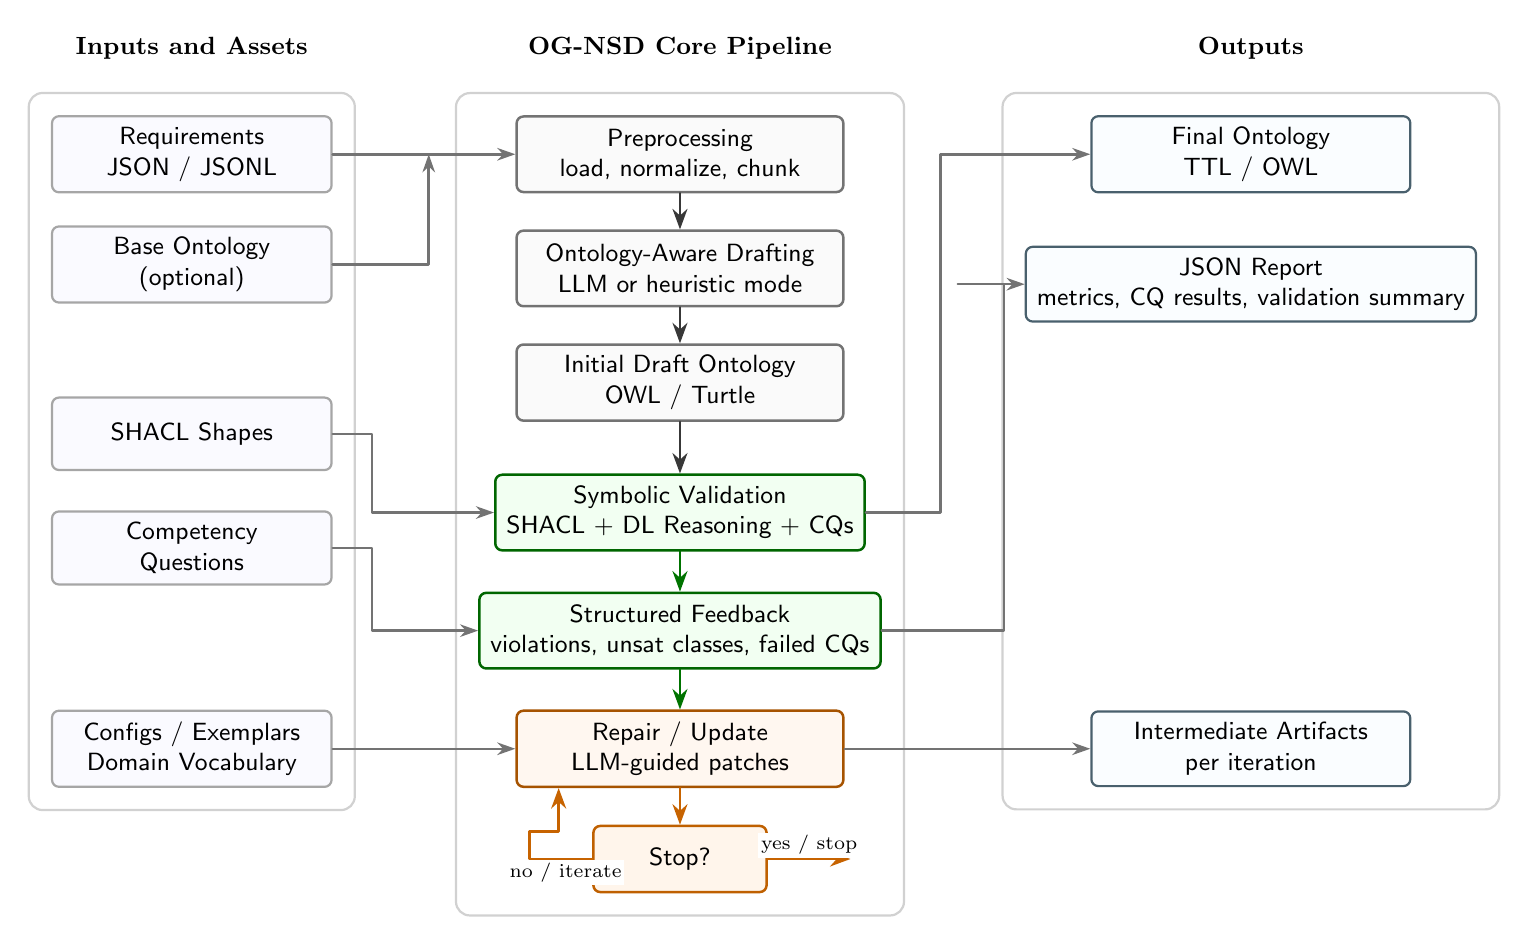
\begin{tikzpicture}[
  font=\sffamily\small,
  >={Stealth[length=2.6mm,width=1.9mm]},
  line join=round,
  line cap=round,
  input/.style={
    rectangle,
    rounded corners=2.5pt,
    draw=black!35,
    fill=blue!2,
    line width=0.8pt,
    minimum width=3.55cm,
    minimum height=0.92cm,
    align=center,
    inner sep=4pt
  },
  core/.style={
    rectangle,
    rounded corners=2.5pt,
    draw=black!55,
    fill=black!2,
    line width=0.9pt,
    minimum width=4.15cm,
    minimum height=0.96cm,
    align=center,
    inner sep=4pt
  },
  validate/.style={
    rectangle,
    rounded corners=2.5pt,
    draw=green!40!black,
    fill=green!5,
    line width=0.9pt,
    minimum width=4.15cm,
    minimum height=0.96cm,
    align=center,
    inner sep=4pt
  },
  repair/.style={
    rectangle,
    rounded corners=2.5pt,
    draw=orange!65!black,
    fill=orange!6,
    line width=0.9pt,
    minimum width=4.15cm,
    minimum height=0.96cm,
    align=center,
    inner sep=4pt
  },
  decision/.style={
    rectangle,
    rounded corners=2.5pt,
    draw=orange!75!black,
    fill=orange!8,
    line width=0.9pt,
    minimum width=2.2cm,
    minimum height=0.84cm,
    align=center,
    inner sep=3pt
  },
  output/.style={
    rectangle,
    rounded corners=2.5pt,
    draw=cyan!35!black,
    fill=cyan!2,
    line width=0.8pt,
    minimum width=4.05cm,
    minimum height=0.92cm,
    align=center,
    inner sep=4pt
  },
  gbox/.style={
    rectangle,
    rounded corners=5pt,
    draw=black!18,
    line width=0.8pt,
    inner sep=8pt
  },
  mainflow/.style={
    -{Stealth[length=2.6mm,width=1.9mm]},
    draw=black!78,
    line width=1.0pt
  },
  auxflow/.style={
    -{Stealth[length=2.3mm,width=1.6mm]},
    draw=black!55,
    line width=0.9pt
  },
  vflow/.style={
    -{Stealth[length=2.6mm,width=1.9mm]},
    draw=green!45!black,
    line width=1.0pt
  },
  rflow/.style={
    -{Stealth[length=2.6mm,width=1.9mm]},
    draw=orange!78!black,
    line width=1.0pt
  },
  sec/.style={font=\bfseries\small},
  looplabel/.style={
    font=\scriptsize,
    fill=white,
    inner sep=1pt
  }
]

% ------------------------------------------------
% Section titles
% ------------------------------------------------
\node[sec] at (0.0,5.95)   {Inputs and Assets};
\node[sec] at (6.20,5.95)  {OG-NSD Core Pipeline};
\node[sec] at (13.45,5.95) {Outputs};

% ------------------------------------------------
% Inputs
% ------------------------------------------------
\node[input] (req)   at (0.0,4.60)  {Requirements\\JSON / JSONL};
\node[input] (base)  at (0.0,3.20)  {Base Ontology\\(optional)};
\node[input] (shacl) at (0.0,1.05)  {SHACL Shapes};
\node[input] (cq)    at (0.0,-0.40) {Competency\\Questions};
\node[input] (cfg)   at (0.0,-2.95) {Configs / Exemplars\\Domain Vocabulary};

% ------------------------------------------------
% Core
% ------------------------------------------------
\node[core]     (prep)     at (6.20,4.60)  {Preprocessing\\load, normalize, chunk};
\node[core]     (draft)    at (6.20,3.15)  {Ontology-Aware Drafting\\LLM or heuristic mode};
\node[core]     (init)     at (6.20,1.70)  {Initial Draft Ontology\\OWL / Turtle};
\node[validate] (valid)    at (6.20,0.05)  {Symbolic Validation\\SHACL + DL Reasoning + CQs};
\node[validate] (feedback) at (6.20,-1.45) {Structured Feedback\\violations, unsat classes, failed CQs};
\node[repair]   (repair)   at (6.20,-2.95) {Repair / Update\\LLM-guided patches};
\node[decision] (stop)     at (6.20,-4.35) {Stop?};

% ------------------------------------------------
% Outputs
% ------------------------------------------------
\node[output] (finalo) at (13.45,4.60) {Final Ontology\\TTL / OWL};
\node[output] (report) at (13.45,2.95) {JSON Report\\metrics, CQ results, validation summary};
\node[output] (interm) at (13.45,-2.95) {Intermediate Artifacts\\per iteration};

% ------------------------------------------------
% Group boxes
% ------------------------------------------------
\node[gbox,fit=(req)(base)(shacl)(cq)(cfg)] {};
\node[gbox,fit=(prep)(draft)(init)(valid)(feedback)(repair)(stop)] {};
\node[gbox,fit=(finalo)(report)(interm)] {};

% ------------------------------------------------
% Main vertical flow
% ------------------------------------------------
\draw[mainflow] (prep.south)     -- (draft.north);
\draw[mainflow] (draft.south)    -- (init.north);
\draw[mainflow] (init.south)     -- (valid.north);
\draw[vflow]    (valid.south)    -- (feedback.north);
\draw[vflow]    (feedback.south) -- (repair.north);
\draw[rflow]    (repair.south)   -- (stop.north);

% ------------------------------------------------
% Stop loop
% ------------------------------------------------
\coordinate (loopL) at ($(stop.west)+(-0.80,0)$);
\coordinate (repairHit) at ($(repair.south west)+(0.55,0)$);
\coordinate (repairBelow) at ($(repairHit)+(0,-0.55)$);

\draw[rflow]
  (stop.west) -- (loopL)
  node[pos=0.42,below,looplabel] {no / iterate}
  |- (repairBelow) -- (repairHit);

\draw[rflow]
  (stop.east) -- ++(1.05,0)
  node[midway,above,looplabel] {yes / stop};

% ------------------------------------------------
% Input routing with common vertical alignment
% ------------------------------------------------
\coordinate (topBus)   at ($(prep.west)+(-1.10,0)$);
\coordinate (inputBus) at ($(valid.west)+(-1.55,0)$);

\coordinate (sTurn) at ($(valid.west)+(-0.85,0)$);
\coordinate (cTurn) at ($(feedback.west)+(-0.85,0)$);
\coordinate (gTurn) at ($(repair.west)+(-0.85,0)$);

\draw[auxflow] (req.east)  -- (topBus |- req.east)  -- (topBus) -- (prep.west);
\draw[auxflow] (base.east) -- (topBus |- base.east) -- (topBus);

\draw[auxflow] (shacl.east) -- (inputBus |- shacl.east) -- (inputBus |- sTurn) -- (sTurn) -- (valid.west);
\draw[auxflow] (cq.east)    -- (inputBus |- cq.east)    -- (inputBus |- cTurn) -- (cTurn) -- (feedback.west);
\draw[auxflow] (cfg.east)   -- (inputBus |- cfg.east)   -- (inputBus |- gTurn) -- (gTurn) -- (repair.west);

% ------------------------------------------------
% Output routing
% ------------------------------------------------
\coordinate (vLane) at ($(valid.east)+(0.95,0)$);
\coordinate (fLane) at ($(feedback.east)+(1.55,0)$);
\coordinate (rLane) at ($(repair.east)+(1.00,0)$);

\coordinate (vTurn) at ($(finalo.west)+(-0.85,0)$);
\coordinate (fTurn) at ($(report.west)+(-0.85,0)$);
\coordinate (rTurn) at ($(interm.west)+(-0.85,0)$);

\draw[auxflow] (valid.east)    -- (vLane) |- (vTurn) -- (finalo.west);
\draw[auxflow] (feedback.east) -- (fLane) |- (fTurn) -- (report.west);
\draw[auxflow] (repair.east)   -- (rLane) -- (rTurn) -- (interm.west);

\end{tikzpicture}}
  \caption{Overview of the OG-NSD pipeline. Natural-language requirements and domain assets are transformed into a draft ontology through ontology-aware drafting. The candidate ontology is then symbolically validated using SHACL, DL reasoning, and competency questions, and iteratively refined through structured feedback until the stopping criteria are satisfied.}
  \label{fig:pipeline}
\end{figure*}

\subsection{Preprocessing}
Preprocessing in OG-NSD is intentionally lightweight. The system performs syntactic loading, whitespace normalization, filtering of empty or malformed entries, and optional chunking of requirement sets. The design avoids aggressive linguistic transformations such as stemming or lemmatization, because the original requirement formulations are treated as the semantic ground truth.

Requirement loading is implemented so that the rest of the pipeline remains format-agnostic. The requirement loader supports both JSONL, where each line is an independent requirement, and JSON lists. In both cases, the output is normalized into a uniform list of strings. Large requirement sets can be chunked into batches in order to respect LLM context limits and to keep execution cost under control. This chunking step functions as an operational split mechanism rather than as a train/validation/test split. It allows the same requirement subset to be used across multiple runs, thus improving reproducibility and comparability.

The same stage also supports the injection of ontology vocabulary and exemplars into prompts. These exemplars are small Turtle fragments that illustrate how requirement phrases should be translated into ontology constructs. They function as a style guide for namespace usage, subclass modeling, and property declarations.

\subsection{Configuration, Model Settings, and Reproducibility}
The behavior of the pipeline is controlled through a unified configuration layer. A configuration object specifies paths to requirements, gold ontologies, SHACL shapes, competency questions, and optional base ontologies, as well as operational parameters such as LLM mode, maximum number of repair iterations, maximum number of requirements to process, whether reasoning is enabled, and whether the run should stop after drafting.

This design supports two desirable properties: reproducibility, because each experiment corresponds to a fixed configuration snapshot, and comparability, because differences between runs can be attributed to explicit parameter changes rather than to hidden code modifications.

The implementation consists of modules for requirement loading and chunking, LLM drafting, ontology parsing and serialization, SHACL validation, DL reasoning, CQ execution, and JSON reporting. The drafting stage supports both a live LLM backend and a heuristic fallback mode. In the reported experiments, the neural baseline explicitly studies two temperatures ($T=0.1$ and $T=0.7$), allowing us to quantify the effect of generation stochasticity. Ontology-aware runs use domain vocabulary and exemplar-guided prompting. Full repair experiments are executed under fixed stopping policies, with maximum iteration budgets defined in the corresponding configuration files. All runs produce serialized ontologies together with JSON summaries, which makes the evolution from initial draft to final output auditable and directly reproducible.

The public implementation and experimental artifacts are available in the project repository at \url{https://github.com/KristiCami/Ontology-Guided}. The released experiment scripts support both OpenAI-backed execution and a deterministic heuristic fallback. In the public code, the effective backend, temperature, ontology-context usage, reasoning flag, and iteration budget are selected through configuration files, while the generated run artifacts record the conditions of each execution. We therefore interpret the reported runs through their configuration snapshots and saved outputs rather than assuming a single fixed backend across all experiments. For the reported OpenAI-backed runs, the provider, model name, decoding settings, and the use of the same or different models across drafting and repair are specified in the corresponding configuration snapshots and documented in the released artifacts.

\subsection{LLM Drafting}
The drafting stage is the neural core of OG-NSD. Its input is a set of normalized requirements, and its output is an initial draft ontology in Turtle. The system supports two execution modes: an OpenAI-backed mode and a heuristic fallback mode. In the public implementation, the effective LLM mode and temperature are selected through configuration, while the heuristic mode remains useful for offline runs and deterministic reproduction.

Ontology-aware prompting is a key feature of the system. When enabled, the pipeline extracts vocabulary from a gold or base ontology---classes, properties, domains, ranges, and prefixes---and injects this information into the prompt as structured context. This does not amount to copying ontology axioms; rather, it acts as a lexical and structural contract that reduces drift and promotes consistent namespace usage. The resulting draft is serialized and stored as a temporary artifact so that its contribution can be studied independently before symbolic correction is applied.

\subsection{Validation and Repair Loop}
After drafting, the candidate ontology is validated at multiple levels.
\begin{itemize}
  \item \textbf{SHACL validation.} SHACL captures structural expectations such as missing properties, invalid typing, incomplete declarations, and domain-specific modeling rules. The resulting violations are fine-grained and interpretable, making them suitable as repair signals.
  \item \textbf{DL reasoning.} Reasoning checks whether the ontology remains logically coherent under OWL semantics. It can reveal inconsistencies and unsatisfiable classes that are not visible through purely local shape checks.
  \item \textbf{Competency-question testing.} Competency questions are implemented as SPARQL ASK queries. They provide an independent signal of domain adequacy by checking whether the ontology supports intended domain questions.
\end{itemize}

The outputs of these validators are then transformed into repair-oriented feedback. Instead of exposing raw tool logs to the model, OG-NSD produces compact structured prompts that specify the problem, its local context, and the expected correction. Let $O^{(t)}$ denote the ontology at iteration $t$. The repair step is written as:
\[
O^{(t+1)}=\mathrm{RepairLLM}(O^{(t)},V_{\mathrm{shacl}}^{(t)},V_{\mathrm{reason}}^{(t)},C^{(t)}),
\]
where $V_{\mathrm{shacl}}^{(t)}$ and $V_{\mathrm{reason}}^{(t)}$ denote validation signals and $C^{(t)}$ denotes optional competency-question feedback.

Each repair iteration includes four substeps: validation, violation aggregation, repair-prompt synthesis, and patch integration into the current graph. The process is therefore closer to counterexample-guided repair than to naive prompt repetition. The entire iteration history is stored in JSON form, making it possible to inspect what changed and why.

\subsection{Termination, Serialization, and Reporting}
The repair loop terminates when no hard SHACL violations remain, when CQ performance stabilizes, when no new patches are produced, or when the maximum number of iterations is reached. These criteria balance quality improvement against runtime and LLM cost.

The final ontology is serialized to Turtle via an ontology abstraction layer built on top of RDFLib. The serialized graph may combine the initial draft, an optional base ontology, and the patches introduced during repair. Intermediate graphs and JSON reports are preserved so that the evolution from draft to final ontology remains fully traceable. As a result, the output of a run is not a single ontology file, but a pair consisting of the final TTL graph and an analytical report containing SHACL summaries, reasoner results, CQ traces, and repair metadata.

\subsection{Robustness and Auditability}
A further implementation detail that is important for interpreting the experiments is that OG-NSD is designed to fail transparently rather than silently. Requirement files are normalized before drafting, Turtle outputs are parsed before downstream validation, and malformed or invalid restrictions are explicitly recorded in the run artifacts rather than being hidden inside later stages. Likewise, intermediate outputs are preserved per iteration so that one can distinguish defects introduced during initial drafting from defects created or amplified during repair.

This matters experimentally for two reasons. First, it improves auditability: when a repair policy behaves poorly, the analyst can inspect the exact draft, validation output, patch set, and post-reasoning graph associated with that run. Second, it improves comparability: because execution is configuration-driven and artifact-producing, differences between methods can be tied to concrete choices such as stopping policy, threshold setting, or prompting mode. In practice, this logging discipline is especially useful in failure cases such as graph explosion, repeated invalid restrictions, or reasoner instability, where a pure black-box evaluation would reveal that something went wrong but not where it went wrong.

\subsection{Evaluation Methodology}
The evaluation of generated ontologies in OG-NSD is explicitly multi-layered. It combines four complementary perspectives.

First, exact matching compares predicted axioms against the reference ontology at strict IRI level after duplicate removal and namespace normalization. Second, we report a relaxed reasoning-aware overlap metric. This metric uses the reasoned graph when reasoning is enabled and otherwise the asserted graph, and compares a normalized schema-oriented triple space. It should therefore be interpreted as an approximate indicator of semantic proximity rather than as full semantic equivalence. Third, structural and logical quality are measured through SHACL and DL reasoning. Fourth, competency questions assess whether the ontology captures the domain knowledge needed to support intended queries.

This layered design is necessary because no single metric captures ontology quality in full. An ontology may be syntactically close to the gold reference while remaining logically weak, or it may be logically valid but still fail to support the intended domain questions.

% \section{Experimental Setup}
\subsection{Domains, Assets, and Research Questions}
The experiments use two domains: ATM and healthcare. Each domain provides requirement files, SHACL shapes, competency questions, and (when available) gold ontologies and base ontologies.

The evaluation is organized around five research questions: (1) whether validation-oriented control improves quality over raw generation, (2) whether ontology-aware prompting improves alignment and structure, (3) whether explicit repair policies add value, (4) whether the same pipeline transfers across domains, and (5) what iterative CQ monitoring reveals.

\subsection{System Variants}
We study six configurations: E1 (neural baseline), E2 (validation-oriented baseline), E3 (ontology-aware drafting), E4 (full OG-NSD with policy variants), E5 (cross-domain transfer), and E6 (CQ-oriented iterative analysis).

\subsection{Metrics}
The evaluation combines exact overlap, relaxed reasoning-aware overlap, SHACL compliance, consistency and reasoner behavior, CQ pass rate, number of predicted triples, overlap count, removed invalid restrictions, missing classes, and graph growth across repair iterations.

% \section{Results}
\subsection{E1: Neural Baseline}
E1 evaluates the system under pure drafting conditions, without SHACL, reasoning, or repair. Two temperature settings are compared.

\subsection{E2 and E3: Validation-Oriented Baseline vs. Ontology-Aware Drafting}
Results suggest that ontology-aware prompting improves lexical alignment and coverage, but not necessarily overall precision.

\subsection{E4: Full OG-NSD with Repair Policies}
Conservative policies preserve a better balance between ontology quality and functional adequacy, whereas aggressive CQ-driven repair increases CQ pass rate at the cost of precision and overall graph quality.

\subsection{E5: Cross-Domain Transfer}
\subsection{E6: CQ-Oriented Iterative Analysis}
E6 acts as an instrumentation view over iterative execution, reporting how CQ pass rate evolves across iterations and when a run reaches a conforming state.

\subsection{Overall Findings}
Low-temperature drafting is a strong baseline; ontology-aware prompting improves lexical alignment but not necessarily precision; iterative repair helps only with controlled stopping policies; CQ-oriented monitoring is diagnostically useful; and cross-domain quality transfer remains limited.

% \section{Discussion}

The main value of OG-NSD is methodological. It reframes ontology drafting as a controlled neuro-symbolic process rather than a one-shot generation problem. This is important for LLM-driven ontology engineering because quality cannot be reduced to fluent output alone; it requires explicit structural, logical, and task-oriented criteria.

The experiments also clarify limits of the approach. Symbolic validation is helpful, but not a universal optimizer. Its benefit depends on how validation feedback is translated into prompts and how termination is controlled. Similarly, competency questions are valuable as adequacy signals, but when treated as the sole optimization target they can encourage overgeneration.

One notable finding is that the best iterative configuration (\texttt{max\_only}) still does not surpass the strongest raw neural baseline (E1 at low temperature) in F1. This does not invalidate the neuro-symbolic framing; rather, it shows that current repair policies privilege structural stabilization over pure overlap maximization.

% \section{Threats to Validity}

Several threats to validity should be acknowledged. \emph{Internal validity} may be affected by prompt sensitivity, implementation choices in the repair loop, and the specific configuration of the LLM backend. \emph{Construct validity} depends on whether SHACL violations, reasoner outcomes, and CQ success adequately capture ontology quality. \emph{External validity} is limited by the number of domains and by reliance on ATM and healthcare assets. \emph{Conclusion validity} depends on stability across seeds, thresholds, model backends, and ontology vocabularies.

In addition, some comparisons involve exact matching and relaxed reasoning-aware matching under different assumptions. These measures are complementary but not interchangeable, and their interpretation must remain tied to the intended evaluation perspective.

% \section{Conclusion}

We presented OG-NSD, a neuro-symbolic pipeline for drafting OWL ontologies from natural-language requirements. The pipeline combines LLM drafting with ontology-aware prompting, SHACL validation, DL reasoning, competency-question checking, and iterative repair.

The study shows that symbolic feedback is useful when it acts as a controlled guidance mechanism, but overly aggressive repair policies can damage precision, destabilize reasoning, and inflate graph size. The most balanced iterative policy in our study is \texttt{max\_only}, while low-temperature neural drafting remains a strong baseline in its own right.

More broadly, the results suggest that the central challenge in LLM-driven ontology engineering is not only how to generate ontologies, but how to regulate the interaction between generation, validation, and stopping.


\begin{thebibliography}{12}

\bibitem{gruber1993}
T. R. Gruber.
A translation approach to portable ontology specifications.
\emph{Knowledge Acquisition}, 5(2):199--220, 1993.

\bibitem{uschold1996}
M. Uschold and M. Gr\"{u}ninger.
Ontologies: Principles, methods and applications.
\emph{The Knowledge Engineering Review}, 11(2):93--136, 1996.

\bibitem{gruninger1995}
M. Gr\"{u}ninger and M. S. Fox.
The role of competency questions in enterprise engineering.
In \emph{Benchmarking --- Theory and Practice}, pages 22--31. Springer, 1995.

\bibitem{monfardini2023}
G. K. Q. Monfardini, J. P. A. Almeida, and G. Guizzardi.
Use of competency questions in ontology engineering: A survey.
\emph{Applied Ontology}, 18(1):1--38, 2023.

\bibitem{shacl2017}
H. Knublauch and D. Kontokostas, editors.
\emph{Shapes Constraint Language (SHACL)}.
W3C Recommendation, 2017.

\bibitem{owl2overview2012}
W3C OWL Working Group.
\emph{OWL 2 Web Ontology Language: Document Overview (Second Edition)}.
W3C Recommendation, 2012.

\bibitem{owl2syntax2012}
B. Motik, P. F. Patel-Schneider, and B. Parsia, editors.
\emph{OWL 2 Web Ontology Language: Structural Specification and Functional-Style Syntax (Second Edition)}.
W3C Recommendation, 2012.

\bibitem{garcia2024thesis}
J. Garc\'{i}a Fern\'{a}ndez.
\emph{Ontology Engineering with Large Language Models}.
Master's thesis, Delft University of Technology / TNO, 2024.

\bibitem{saeedizade2024}
M. J. Saeedizade, A. S. Lippolis, M. Poveda-Villal\'{o}n, and O. Corcho.
Navigating ontology development with large language models.
In \emph{Proceedings of ESWC 2024 Workshops}, 2024.

\bibitem{lippolis2024}
A. S. Lippolis, M. J. Saeedizade, M. Poveda-Villal\'{o}n, and O. Corcho.
Ontology generation with metacognitive prompting in large language models.
In \emph{Proceedings of ESWC 2024 Workshops}, 2024.

\bibitem{garijo2025}
D. Garijo, M. Poveda-Villal\'{o}n, E. Amador-Dom\'{i}nguez, Z. Wang, R. Garc\'{i}a-Castro, and O. Corcho.
LLMs for ontology engineering: A landscape of tasks and benchmarking challenges.
In \emph{Proceedings of the 1st International Workshop on LLMs for Ontology Engineering}, 2025.

\bibitem{delong2024}
L. N. DeLong, R. Fern\'{a}ndez Mir, and J. D. Fleuriot.
Neurosymbolic AI for reasoning over knowledge graphs: A survey.
\emph{arXiv preprint arXiv:2302.07200}, 2024.

\end{thebibliography}


\end{document}

